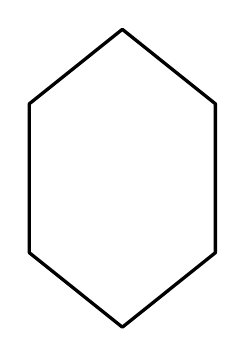
\begin{tikzpicture}[line cap=round, line join=round, line width=1.2pt, scale=1]

% This matches the picture better than a perfect regular hexagon:
% - same vertex orientation (pointed top/bottom)
% - slightly taller (vertical stretch), slightly narrower (horizontal squeeze)

\def\R{1.55} % overall size

\begin{scope}[xscale=0.88, yscale=1.22] % shape tuning to match the scan
  % Vertices (point-up hexagon)
  \coordinate (A) at (90:\R);    % top
  \coordinate (B) at (30:\R);    % upper-right
  \coordinate (C) at (-30:\R);   % lower-right
  \coordinate (D) at (-90:\R);   % bottom
  \coordinate (E) at (-150:\R);  % lower-left
  \coordinate (F) at (150:\R);   % upper-left

  % Draw hexagon
  \draw (A)--(B)--(C)--(D)--(E)--(F)--cycle;
\end{scope}

\end{tikzpicture}